\documentclass[12pt]{article}
\usepackage{amsmath}
\usepackage{scrextend}
\usepackage{graphicx}
\usepackage[margin=1.0in]{geometry}
\graphicspath{ {images/} }
\begin{document}

\title{Classification of Printed Digits}
\author{Riley Tuttle\\
ELE665}
\renewcommand{\today}{May 3, 2017}
\maketitle
%preamble
%%%%%%%%%%%%%%%%%%%%%%%%%%%%%%%%%%%%%%%%%%%%%%%%%%%%%%%%%%%%%%%%%%%%%%%%%%%%%%%%%%%%%%%%%
\section {Goal}
	The goal of this project is to develop a detector to classify printed digits in a frame.
	There will be a few different problems addressed in this report.
	All of these problems will be multiple hypothesis classification problems because the 		image can be any of 10 different digits.
	The case of no digit will be ignored in this project.
	Each problem will assume less and less is known about the digit.
%%%%%%%%%%%%%%%%%%%%%%%%%%%%%%%%%%%%%%%%%%%%%%%%%%%%%%%%%%%%%%%%%%%%%%%%%%%%%%%%%%%%%%%%%
\section{Digits}
	Each digit will be a 5x5 pixel image set in a 20x20 pixel frame as can be seen seen
		in figure \ref{fig:digits}.
	Each pixel will be considered centered in the 20x20 frame such that the top left pixel
		of the 5x5 pixel digit is located at frame pixel location (7,7) as seen in figure
		\ref{fig:centeredDigit}
	The pixel location will be considered as a coordinate plane with origin in the top left
		corner and the y axis will be positive when counting from top to bottom.
	\begin{figure}[h]
		\centering
		
\includegraphics[width=0.75\textwidth]{centeredDigit.png}
		\caption{The number 3 centered at frame location (7,7).}
		\label{fig:centeredDigit}
	\end{figure}
	Each pixel will be grayscale from 0 to 255.
	Without any noise the color of the digit will be in the middle at 127 and the
		background will be 0.
	For each Problem there will be 5000 test digits to test the detector's simulated
		performance.
	\begin{figure}[b]
		\centering
		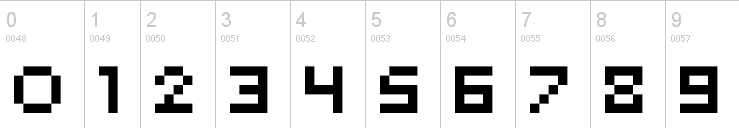
\includegraphics[width=\textwidth]{digits.png}
		\caption{5x5 digits.}
		\label{fig:digits}
	\end{figure}
%%%%%%%%%%%%%%%%%%%%%%%%%%%%%%%%%%%%%%%%%%%%%%%%%%%%%%%%%%%%%%%%%%%%%%%%%%%%%%%%%%%%%%%%%
\section{Problem of known digits}
	The first trivial detector assumes no noise nor any kind of distortion.
	This detector is simply a classifer for the 10 possible digits (signals).
	We look at the data as a vector of 400 (20x20) values to make calculations easier.
	The problem then becomes:
	\begin{gather*}
		\text{Under} \ \mathcal{H}_i: X[n] = s_i[n] \\
		i = 1,2,...,10 \ n=1,2,...,400
	\end{gather*}
	In order to avoid indexing problems with matlab $i = 10$ refers to digit "0".
	Because everything is known and there is no noise a special case of the minimum
		distance receiver can be used to classify the images.
	We would decide $\mathcal{H}_i$ for which:
	\begin{gather*}
		T(x) = \sum_{n=0}^{N-1}x[n]-s[n] = \gamma' = 0;
	\end{gather*}
	Since there is no noise and I would expect perfect detection and in fact I am not
		even going to simulate this.
	Instead I will move on to a more interesting detector.
	
	
		%\begin{equation}
		%\text{Under} \mathcal{H}_i$: $X[n] = s_i[n] + w[n] \\
		%i = 1,2,...,10 \ n=1,2,...,400\\
		%\text{where} w[n] \text{is} \sim \mathcal{N}(127,127
	%\end{equation}
%%%%%%%%%%%%%%%%%%%%%%%%%%%%%%%%%%%%%%%%%%%%%%%%%%%%%%%%%%%%%%%%%%%%%%%%%%%%%%%%%%%%%%%%%
\section{Problem of digits embedded in noise}
	For the first real detector we assume that we know each digit exactly along with its 			size and location in the frame.
	The unknowns are the color of each pixel and of course which digit it is.
	The color of the pixel will be a RV with an approximate distribution $\sim \mathcal{N}
		(127,127)$ under $\mathcal{H}_f$ and $\sim \mathcal{N}(0,127)$ under
		$\mathcal{H}_b$ (where $\mathcal{H}_f$ refers to a pixel that is part of
		the image foreground picture and $\mathcal{H}_b$ refers to a pixel that is
		part of the image background.
	Those distributions are approximate because the values need to be constrained to be 		between 0 and 255.\\
	\\
	Similiar to the previous section we have:
	\begin{gather*}
		\text{Under} \ \mathcal{H}_i: X[n] = s_i[n] + w[n] \\
		i = 1,2,...,10 \ n=1,2,...,400
	\end{gather*}
	Notice the noise added to the signal. Where the noise $w[n] \sim \mathcal{N}(127,127)$.
	This problem is solved using a Minimum Distance Receiver as outlined in section 4.5.1
		and example 4.6 of the book.
	We decide $\mathcal{H}_i$ for which:
	\begin{gather*}
		T_i(x) = \sum_{n=1}^{N}x[n]s_i[n]-\frac{1}{2}\epsilon_i
	\end{gather*}
	is maximum.
	Since this is a case of 10 hypotheses the calculation for probability of error $P_e$
		will be difficult to calculate but I can provide a upper bound on the error using
		equation (4.28) from the book.
	equation (4.28) assumes the same energy $\epsilon$ for each hypothesis in order to 
		simplify calculation but if they are all different the error will go down.
	\begin{equation}
		P_e = 1-\int_{-\infty}^{\infty}
		\Phi^{M-1}(u)
		\frac{1}{\sqrt{2\pi}}
		exp[-\frac{1}{2}(u-\sqrt{\frac{\epsilon}{\sigma^2}})^2] \ du
	\end{equation}
	where $u = (t+\frac{1}{2})/\sqrt{\sigma^2\epsilon}$.
	My simulation error was $P_e = 0$.
	
	%Each digit based on  to develop a detector to detect one or more "target" 
	%	pixels in a 20 by 20 frame that may contain a target.
	%A pixel with no target has WGN distribution with $\sigma^2 = 2$ and a
	%target pixel also has a WGN distribution with $\sigma^2 = 2.75$ such that:\\
	%\begin{addmargin}{2em}
	%	Under $\mathcal{H}_0$: $X[m,n,k] \sim N(0,2)$\\
	%	Under $\mathcal{H}_1$: $X[m,n,k] \sim N(0,2.75)$\\
	%	where $m,n = 1,2,...,20, \ k = 1,2,...,100$
	%\end{addmargin}
%%%%%%%%%%%%%%%%%%%%%%%%%%%%%%%%%%%%%%%%%%%%%%%%%%%%%%%%%%%%%%%%%%%%%%%%%%%%%%%%%%%%%%%%%
\section{Problem of unknown digit location embedded in noise}
	For this problem we assume that the digit can be anywhere inside the frame such that
		the entire digit is still contained in the frame.
	This means that in addition to the noise in the color the digit can have a shift
		that is distributed as $\sim \mathcal{N}(.5,7.5)$ in both the X and Y direction.
	Again this distribution is approximate because the digit needed to be constrained to
		the frame and pixels are discrete.
	This becomes a problem of unknown arrival time but in 2 dimensions so that
	\begin{gather*}
		\text{Under} \ \mathcal{H}_i: X[n] = s_i[n-n_0,m-m_0] + w[n] \\
		i = 1,2,...,10 \ n,m=1,2,...,20 \ n_0,m_0 \in 1,2,...,16
	\end{gather*}
	The GLRT statistic then becomes a maximization of the test statistic over the
		arrival time parameters:
	\begin{equation}
		T(x) = \sum_{n=0}^{N-1}x[n]s_i[n] -\frac{1}{2}\epsilon_i
	\end{equation}
	becomes:
	\begin{gather*}
		T_i(x) = \underset{n_0,m_0 \in 1,16}{\text{max}}\sum_{n=n_0,m=m_0}^{n=N-1,m=M-1} 
		x[n]s_i[n,m] - \frac{\epsilon_i}{2} \\
		N,M = 20
	\end{gather*}
	Then we decide $H_i$ for which $T_i(x)$ is maximum.
	Finding the performance of this classifier is difficult because the signals at 
		different	arrivals are correlated.
	Finding the maximum of a sum of correlated signals is difficult.
	My simulated $P_e$ was $0.0132$ which equates to 66 incorrect decisions out of 5000.
%%%%%%%%%%%%%%%%%%%%%%%%%%%%%%%%%%%%%%%%%%%%%%%%%%%%%%%%%%%%%%%%%%%%%%%%%%%%%%%%%%%%%%%%%
\section{Problem of unknown digit size}
	For this problem each digit has a scale that is distributed as $\sim\mathcal{U}(1,3)$.
	The process I used to scale digits assumes discrete scales so as to avoid dealing
		with interpolation.
	In a future version of the project a different scaling algorithm could be developed
		takes interpolation into account.
	The upper bound of scaling is 3 because the any larger scaling factors would produce
		digits that are larger than the 20x20 frame.
	This problem ends up being very similar to the previous one.
 	In fact it is the same detector maximized over the scaling parameter instead of the
		translation parameters such that we decide $\mathcal{H}_i$ for which:
	\begin{gather*}
		T_i(x) = \underset{s \in 1,3}{\text{max}}\sum_{n=0}^{N-1} 
		x[n]s_i[n,s] - \frac{\epsilon_i}{2} \\
	\end{gather*}
	It is important to remember that s is not an amplitude because scaling a digit
		changes the nature of the signal.
	My simulated $P_e$ was 0.
	I think it makes sense to have have a smaller $P_e$ in comparison to the problem of 
		unknown location because when the digits are larger but the frame remains the same
		size, thus the energy to noise ratio is increased.
%%%%%%%%%%%%%%%%%%%%%%%%%%%%%%%%%%%%%%%%%%%%%%%%%%%%%%%%%%%%%%%%%%%%%%%%%%%%%%%%%%%%%%%%%
\section{Problem of unknown digit size and location}
	Again this problem is just an extension of the previous 2 problems.
	The detector simply maximizes over the translation paramters as well as the scaling
		parameters.
	After simulating the $P_e$ was .0022 which equates to about 11 errors out 5000.
%%%%%%%%%%%%%%%%%%%%%%%%%%%%%%%%%%%%%%%%%%%%%%%%%%%%%%%%%%%%%%%%%%%%%%%%%%%%%%%%%%%%%%%%%
\section{Problem of unknown size, location, and rotation}
	This problem assumes the same unknowns as the previous problem with the added unknown
		rotation parameter.
	The rotations of the digits are distributed as $\sim\mathcal{U}(-\frac{\pi}{4},\frac{\pi}{4})$
		in radians.
	For the same reason that the scaling process was very limited the rotation process is
		very approximate.
	The rotation process does not interpolate at all so some of the images can be good
		(see figure \ref{fig:goodRotation}) and some can look very skewed (see figure
		\ref{fig:badRotation}).
	\begin{figure}[h]
		\centering
		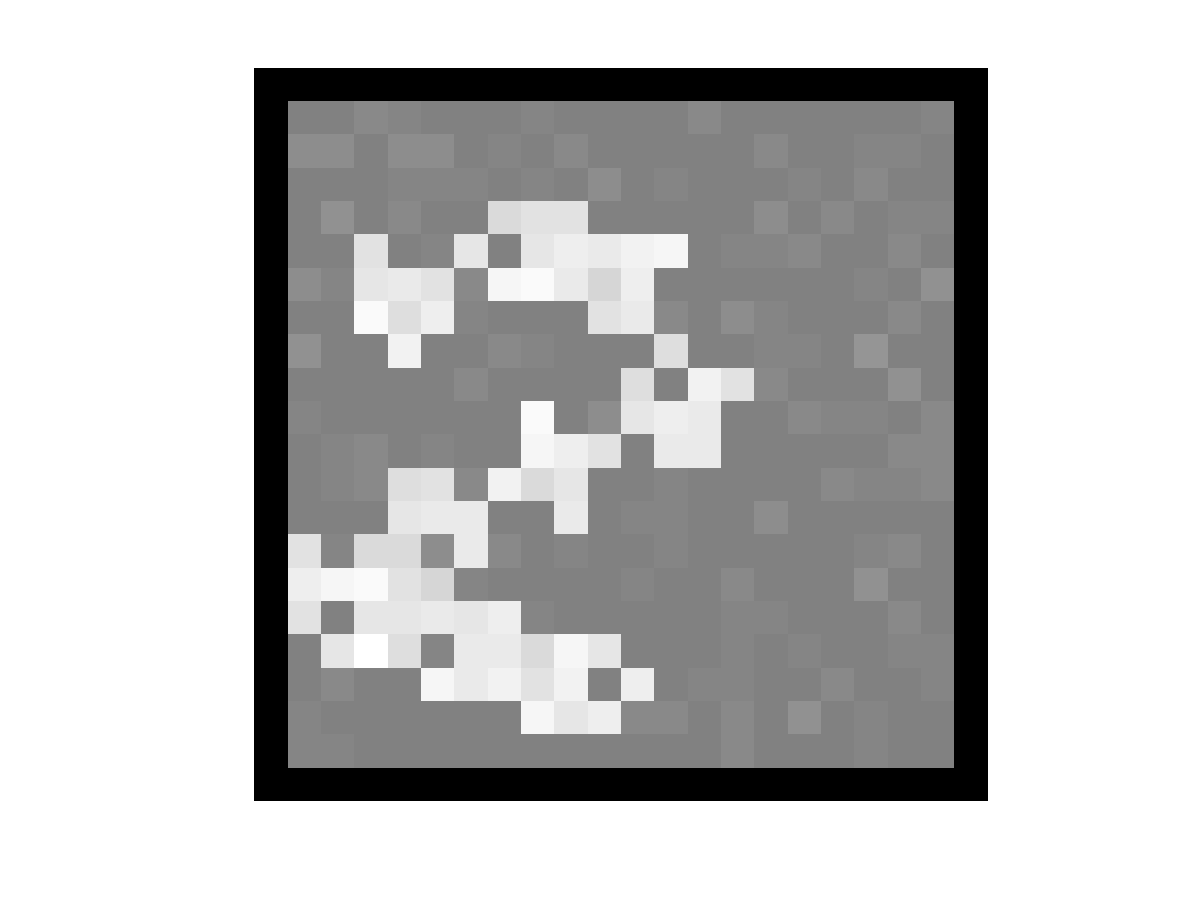
\includegraphics[width=0.75\textwidth]{goodRotation.png}
		\caption{An example of a good rotation.}
		\label{fig:goodRotation}
	\end{figure}
	\begin{figure}[h]
		\centering
		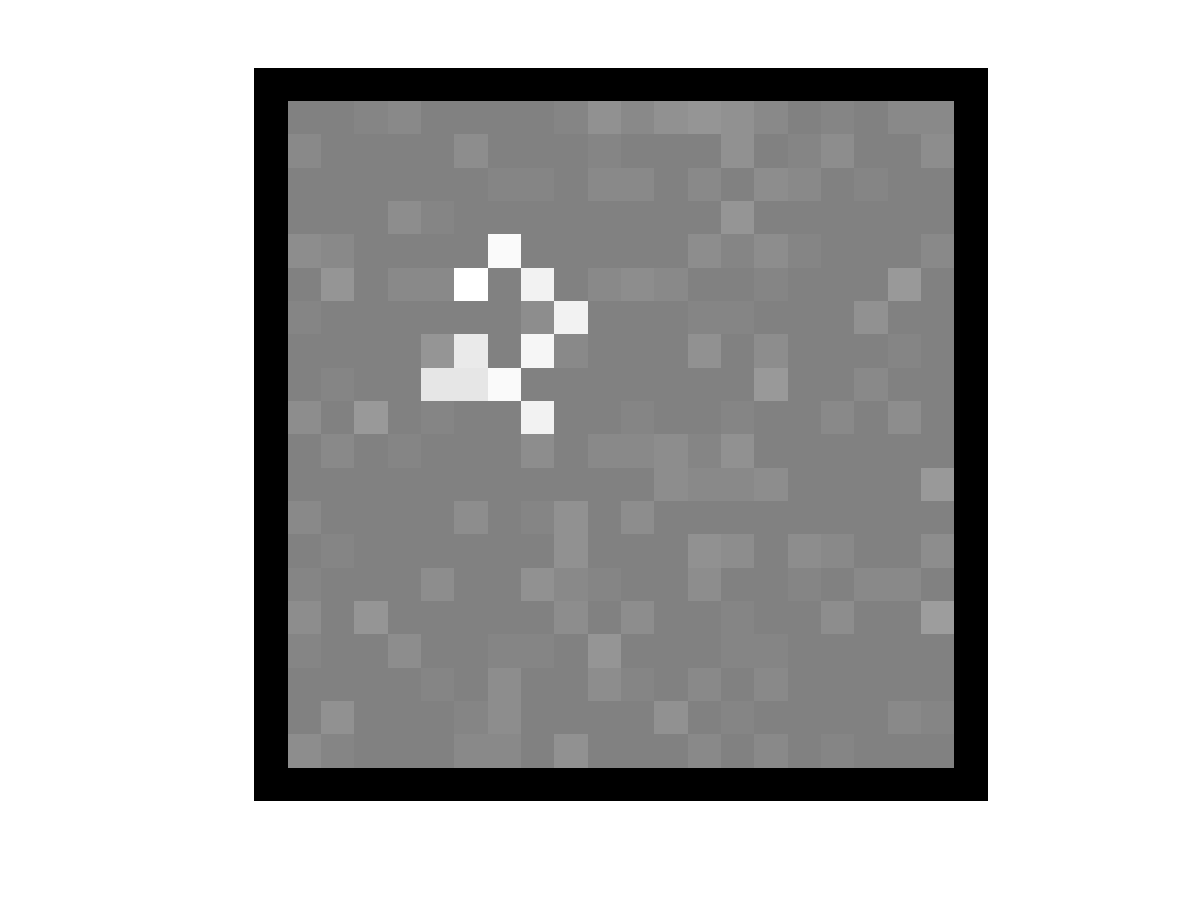
\includegraphics[width=0.75\textwidth]{badRotation.png}
		\caption{An example of a bad rotation.}
		\label{fig:badRotation}
	\end{figure}
	That being said, the detector is again very similar to the previous ones, it just
		maximizes over another parameter set such that we decide $\mathcal{H}_i$ for which:
	\begin{gather}
		T_i(x) = \underset{n_0,m_0 \in 1,16 \ s \in 1,3 \ r \in -\frac{\pi}{4},\frac{\pi}{4}}{\text{max}}
		\sum_{n=n_0,m=m_0}^{n=N-1,m=M-1}
		x[n]s_i[n,m,s,r] - \frac{\epsilon_{i,s,r}}{2} \\
		N,M = 20 \nonumber
		\label{equation:loc_siz_rot}
	\end{gather}
	After using this detector my simulated performance $P_e$ was .0076 which 
		equates to 38 errors out of 5000.
%%%%%%%%%%%%%%%%%%%%%%%%%%%%%%%%%%%%%%%%%%%%%%%%%%%%%%%%%%%%%%%%%%%%%%%%%%%%%%%%%%%%%%%%%
\section{Problem of written digits}
	For all the previous problems the detector didn not really change between them, it just
		maximizes over more and more parameters.
	What's more is that I generated the data,	and classified using the
		same translation, scaling and rotation processes, so of
		course my error rates are going to be low i.e. $P_e < .05$.
	In order to give the detector a real test I wanted to use it on more challenging
		data set.
	For this problem I have a set of 5000 written digits that I want to classify.
	A sample of those digits can be seen in figure \ref{fig:writtenDigits}.
	After just applying the same detector from the previous section I get a $P_e = .6884$.
	That is not very good but considering that random classification would result in a 
		$P_e = .9$ it becomes comparably much better.
	One thing that might be noticed when comparing the printed digits to the written
		digits is the difference in edges.
	The printed digits have "sharp" edges as in they will have potentially very large
		differences in adjacent pixels whereas the written digits are a little bit smoother.
	So as an extension of this detector I first smoothed the template digit.
	That means running every $s[n,m,s,r]$ from equation %\ref{equation:loc_siz_rot}
		3 through a simple 3x3 pixel averager.
	After using this detector with blurred templates my simulated performance was 
		was decreased to $P_e =.5174$.
	Again that is not very good but it is much better than random chance of $P_e = .9$ and
		it is even significantly better than the previous $P_e = .6884$ with about a $17\%$
		improvement.
	A breakdown of the perfomance can be seen in figure \ref{fig:resultsbreakdown}.
	The rows of figure \ref{fig:resultsbreakdown} represent what the digit was and the 
		columns represent what the detector chose.
	So all the rows should sum up to 500 because there were 500 of each digit.
	An example of reading the table is as follows:
	Looking only at row '2' would be looking at all the sample digits that were actually
		'2'.
	The detector falsly classified the digit '2' as the digit '1' 79 times.
	It correctly classified it 207 times. 
	It falsly classified the digit '2' as the digit '3' 68 times so on and so forth.
	As can be seen the detector classifies almost perfectly all the '1's. A lot of '6's
		got classified as '5's.
	That makes sense because those digits look pretty similar.
	I'm guessing that very few things got classified as '8's because the templates had more
		power than any written digits had.
	Because the template for '8' has a high energy the energy compensation term of
		$-\frac{\epsilon}{2}$ would drive down the test statistic of any potential
		'8's causing them to be classified as something else.
	I would speculate that is because most people draw '8's as more slender than a printed
		'8' would look leading to a template that has much more energy than the written 
		digit.
	I think that the classifier could perform even better if I was to develop more 
		robust translation, scaling, and rotation processes that incorporated interpolation.
	However I will note that at that point it might take prohibitively long to do the
		calculations for even this relatively small (5000 samples) data set.
	At that point a different approach, perhaps involving machine learning,
		might be better suited for this problem.
	\begin{figure}[h]
		\centering
		
\includegraphics[width=\textwidth]{writtenDigits.png}
		\caption{A sampling of the written digits.}
		\label{fig:writtenDigits}
	\end{figure}
	\begin{figure}[h]
		\centering
		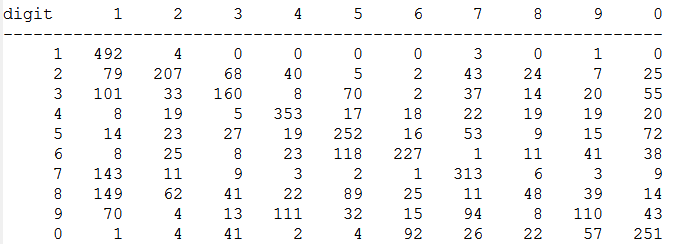
\includegraphics[width=\textwidth]{resultbreakdown.png}
		\caption{A breakdown of the results for classifying written digits with
		blurred templates.}
		\label{fig:resultsbreakdown}
	\end{figure}
%%%%%%%%%%%%%%%%%%%%%%%%%%%%%%%%%%%%%%%%%%%%%%%%%%%%%%%%%%%%%%%%%%%%%%%%%%%%%%%%%%%%%%%%%
\pagebreak
%%%%%%%%%%%%%%%%%%%%%%%%%%%%%%%%%%%%%%%%%%%%%%%%%%%%%%%%%%%%%%%%%%%%%%%%%%%%%%%%%%%%%%%%%
%\section{APPENDIX A}
%	\includegraphics[width=\textwidth]{.png}
\end{document}
